\chapter{Základní problematika amortizované složitosti}
Druhá kapitola se věnuje základní problematice amortizované složitosti a pojmům, které s ní úzce souvisejí. Nejprve shrnuje obecné principy analýzy algoritmů a pojem časové složitosti, které tvoří východisko pro pochopení amortizované analýzy. Následně vysvětluje význam amortizované složitosti a ukazuje, proč není vždy vhodné hodnotit efektivitu algoritmu pouze podle nákladů jedné samostatné operace. Dále představuje základní metody amortizované analýzy se zvláštním důrazem na potenciálovou metodu. V závěru kapitoly je zařazen také stručný přehled algoritmů, u nichž lze amortizovanou analýzu využít, včetně algoritmů vybraných do praktické části této práce.



\section{Základní pojmy analýzy algoritmů}
V této části jsou stručně vymezeny základní pojmy analýzy algoritmů a naznačena jejich návaznost na amortizovanou analýzu.

\subsection{Vymezení základních pojmů}
Analýza algoritmů spočívá ve zkoumání vlastností algoritmů, především jejich správnosti a náročnosti výpočtu. V běžné praxi bývá přesné vyjádření složitosti obtížné, protože závisí na konkrétním výpočetním modelu i na konkrétní implementaci algoritmu. Z tohoto důvodu se v teorii algoritmů využívá asymptotické vyjadřování, které potlačuje méně podstatné detaily a umožňuje soustředit se především na to, jak rychle roste náročnost algoritmu se zvětšující se velikostí vstupu \cite{sawa_ti_03}.

Mezi nejzákladnější pojmy, které se v analýze algoritmů běžně používají, patří algoritmus, vstup, výstup, korektnost a složitost. Algoritmus lze chápat jako přesně definovaný postup, který vede od vstupních dat k požadovanému výsledku. Vstup představuje data, nad nimiž je algoritmus vykonáván, zatímco výstup je výsledkem jejich zpracování. Korektnost vyjadřuje, zda algoritmus pro přípustný vstup poskytuje správný výstup, zatímco složitost popisuje, jaké množství prostředků je potřeba k dosažení výsledku. Teprve kombinace těchto hledisek umožňuje smysluplně hodnotit kvalitu navrženého řešení.

\subsection{Přehled základních charakteristik algoritmů}
Pro lepší přehlednost shrnuje tabulka \ref{tab:basic_terms_algorithm_analysis} vybrané základní pojmy, se kterými se v rámci analýzy algoritmů dále pracuje.

\begin{table}[H]
\centering
\caption{Základní pojmy používané při analýze algoritmů}
\label{tab:basic_terms_algorithm_analysis}
\begin{tabular}{|p{3.2cm}|p{8.5cm}|}
\hline
\textbf{Pojem} & \textbf{Stručné vysvětlení} \\ \hline
    Algoritmus & Jednoznačně definovaný postup, který převádí vstupní data na požadovaný výstup. \\ \hline
    Vstup & Data, nad nimiž je algoritmus vykonáván. Velikost vstupu obvykle ovlivňuje náročnost výpočtu. \\ \hline
    Výstup & Výsledek zpracování vstupu algoritmem. \\ \hline
    Korektnost & Vlastnost algoritmu, která určuje, zda algoritmus poskytuje správný výsledek pro přípustné vstupy. \\ \hline
    Časová složitost & Vyjadřuje náročnost algoritmu z hlediska času, resp. počtu provedených operací. \\ \hline
    Paměťová složitost & Vyjadřuje nároky algoritmu na paměť během výpočtu. \\ \hline
    Asymptotické vyjádření & Způsob popisu růstu náročnosti algoritmu pro velké vstupy bez zdůrazňování méně podstatných detailů. \\ \hline
\end{tabular}
\end{table}

\subsection{Návaznost na amortizovanou analýzu}
Pro potřeby této práce je podstatné, že u některých datových struktur a algoritmů nemusí samostatné hodnocení jedné operace dostatečně vystihnout skutečné chování celého řešení. V takových situacích je vhodné sledovat náklady celé posloupnosti operací, což je princip, na němž je založena amortizovaná analýza \cite{kozen_amortized}. Tento přístup je podrobněji vysvětlen v následujících částech kapitoly.

\newpage

\section{Časová složitost algoritmů}
V této části je nejprve vysvětlen pojem velikosti vstupu a základní způsob vyjádření časové složitosti algoritmu. Následně je pozornost věnována časové složitosti v nejhorším a průměrném případě, asymptotické notaci a vybraným třídám růstu funkcí. Závěr této části ukazuje praktický význam časové složitosti při porovnávání algoritmů a její vztah k amortizované analýze.

\subsection{Velikost vstupu a definice časové složitosti}
Časová složitost algoritmů patří mezi nejdůležitější charakteristiky používané při hodnocení efektivity algoritmických řešení. Počítače sice pracují velmi rychle, jejich výpočetní možnosti však nejsou neomezené, a proto i provedení jednotlivých instrukcí vyžaduje určitý čas. Stejný problém navíc může být řešen více různými algoritmy, jejichž doba výpočtu se může výrazně lišit. Z tohoto důvodu je vhodné algoritmy mezi sebou porovnávat a zkoumat jejich náročnost z hlediska počtu provedených operací \cite{sawa_ti_03}.

Při běžném programování je sice možné algoritmus implementovat a následně změřit dobu jeho běhu na konkrétních vstupních datech, takový přístup však neposkytuje dostatečně obecnou informaci o chování algoritmu pro všechny možné vstupy. V teorii algoritmů se proto časová složitost nevyjadřuje přímo pomocí skutečného času naměřeného na konkrétním zařízení, ale spíše pomocí počtu provedených instrukcí nebo elementárních operací. Díky tomu je možné odhlédnout od konkrétního hardwaru a zaměřit se na samotné chování algoritmu \cite{sawa_ti_03}.

Důležitým pojmem při analýze časové složitosti je velikost vstupu. Pro různé typy problémů může být definována různě. Například u problému třídění lze za velikost vstupu považovat počet prvků ve vstupní posloupnosti, u problémů pracujících s čísly může být přirozenější zvolit počet bitů potřebných k jejich zápisu a u grafových problémů lze velikost vstupu vyjádřit například dvojicí hodnot udávajících počet vrcholů a počet hran. Zvolená definice velikosti vstupu tedy není vždy pevně dána, ale měla by přirozeně odpovídat povaze analyzovaného problému \cite{sawa_ti_03}.

Uvažujme nyní konkrétní algoritmus a jeho implementaci. Pro vstupy stejné velikosti nemusí algoritmus vždy vykonat stejný počet instrukcí, protože jeho chování může záviset na konkrétním uspořádání vstupních dat. Proto se v teorii často zavádí funkce \(T(n)\), která pro každou velikost vstupu \(n\) udává maximální počet instrukcí provedených algoritmem na vstupu velikosti \(n\). Takto definovaná funkce představuje časovou složitost algoritmu v nejhorším případě a umožňuje zachytit horní mez výpočetní náročnosti \cite{sawa_ti_03}.

\newpage

\subsection{Časová složitost v nejhorším a průměrném případě}
Pro lepší názornost je princip časové složitosti v nejhorším případě znázorněn na obrázku \ref{fig:worst_case_complexity}. Jednotlivé body představují různé vstupy stejné nebo podobné velikosti a jejich skutečnou časovou náročnost. Funkce \(T(n)\) zde odpovídá horní hranici těchto hodnot, tedy nejhoršímu případu pro danou velikost vstupu.

\begin{figure}[H]
    \centering
    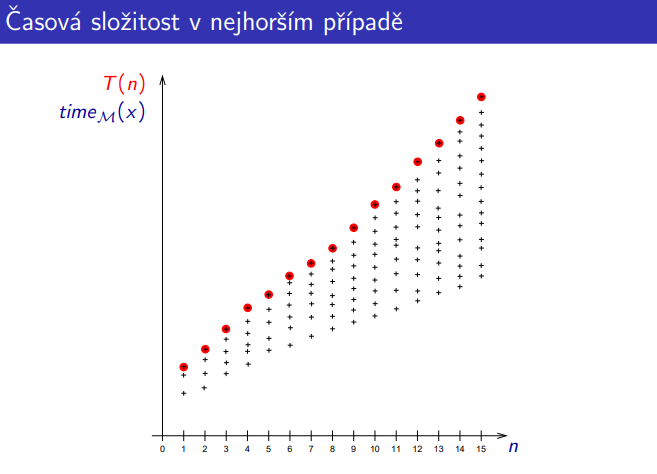
\includegraphics[width=0.78\textwidth]{Figures/worst_case.png}
    \caption{Časová složitost v nejhorším případě podle \cite{sawa_ti_03}}
    \label{fig:worst_case_complexity}
\end{figure}

Obrázek \ref{fig:worst_case_complexity} ukazuje, že pro vstupy stejné velikosti nemusí algoritmus vždy vykonat stejný počet operací. Časová složitost v nejhorším případě proto sleduje maximální hodnotu těchto nákladů a poskytuje tak bezpečný odhad horní meze časové náročnosti algoritmu.

Vedle časové složitosti v nejhorším případě má smysl zkoumat také časovou složitost v průměrném případě. V tomto případě není funkce \(T(n)\) určena maximální hodnotou přes všechny vstupy dané velikosti, ale aritmetickým průměrem odpovídajících nákladů. Určení průměrného případu však bývá zpravidla obtížnější než určení nejhoršího případu, protože vyžaduje přesnější představu o množině vstupů a jejich rozdělení. Ve většině případů se proto při analýze algoritmů častěji vychází právě z nejhoršího případu \cite{sawa_ti_03}.

Pro názornost je na obrázku \ref{fig:average_case_complexity} znázorněna časová složitost v průměrném případě. Na rozdíl od nejhoršího případu zde funkce \(T(n)\) nepředstavuje horní obálku všech hodnot, ale jejich průměrné chování pro vstupy stejné velikosti.

\begin{figure}[H]
    \centering
    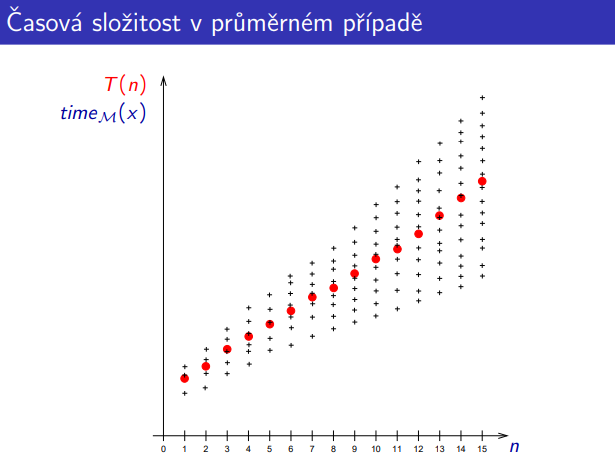
\includegraphics[width=0.78\textwidth]{Figures/average_case.png}
    \caption{Časová složitost v průměrném případě podle \cite{sawa_ti_03}}
    \label{fig:average_case_complexity}
\end{figure}

Časová složitost v nejhorším a průměrném případě se často příliš neliší, i když v některých situacích může být rozdíl významný. Zároveň se uvádí, že zkoumání složitosti v nejlepším případě obvykle nemá příliš velký praktický význam \cite{sawa_ti_03}.

\newpage

\subsection{Asymptotická notace a třídy růstu funkcí}
Přesné vyjádření časové složitosti bývá často komplikované a silně závisí na zvoleném výpočetním modelu i na detailech implementace. Ve většině případů navíc není nutné znát přesný počet instrukcí, ale stačí odhadnout, jak rychle tento počet roste se zvětšující se velikostí vstupu. Právě z tohoto důvodu se zavádí asymptotická notace, která zanedbává méně podstatné detaily a umožňuje soustředit se na dominantní složku růstu sledované funkce \cite{sawa_ti_03}.

V rámci asymptotické notace se nejčastěji používají symboly \(O\), \(\Omega\) a \(\Theta\). Zápis \(O(g(n))\) vyjadřuje horní asymptotickou mez růstu funkce, tedy skutečnost, že sledovaná funkce neroste rychleji než funkce \(g(n)\) až na konstantní násobek. Naopak \(\Omega(g(n))\) vyjadřuje dolní asymptotickou mez a \(\Theta(g(n))\) charakterizuje situaci, kdy funkce roste stejnou rychlostí jako \(g(n)\) z hlediska horní i dolní meze současně. Kromě těchto symbolů se používají také \(o(g(n))\) a \(\omega(g(n))\), které popisují přísně pomalejší, respektive přísně rychlejší růst \cite{sawa_ti_03}.

Big-O notace popisuje asymptotické chování funkcí a umožňuje při analýze algoritmů zanedbat konstanty i pomaleji rostoucí členy \cite{mit_big_o}. Mezi běžné třídy patří například \(O(1)\), \(O(\log n)\), \(O(n)\), \(O(n^2)\), polynomiální růst a exponenciální růst, přičemž exponenciální funkce rostou výrazně rychleji než funkce polynomiální \cite{mit_big_o}.

Na základě asymptotického chování lze algoritmy rozdělovat do několika základních tříd. Za logaritmické se považují algoritmy se složitostí \(\Theta(\log n)\), za lineární algoritmy se složitostí \(\Theta(n)\), za kvadratické se považují algoritmy se složitostí \(\Theta(n^2)\) a podobně. Významnou skupinu tvoří také polynomiální algoritmy, tedy algoritmy, jejichž časová složitost je shora omezena nějakým polynomem. Naopak exponenciální nebo faktoriální složitosti obvykle vedou k tomu, že algoritmus je použitelný pouze pro velmi malé vstupy \cite{sawa_ti_03,mit_big_o}.

Praktický význam rozdílné rychlosti růstu funkcí ukazuje tabulka \ref{tab:growth_rate_functions}. Ta vychází z předpokladu, že algoritmus zpracovává vstup velikosti \(n\), provede \(T(n)\) operací a provedení jedné operace trvá \(1\,\mu s\). Je z ní patrné, že rozdíly mezi jednotlivými třídami složitosti se s rostoucí velikostí vstupu velmi rychle zvětšují \cite{sawa_ti_03}.

\begin{table}[H]
\centering
\caption{Příklad růstu doby výpočtu pro vybrané třídy časové složitosti podle \cite{sawa_ti_03}}
\label{tab:growth_rate_functions}

\setlength{\tabcolsep}{3pt}
\renewcommand{\arraystretch}{1.15}
\scriptsize

\resizebox{\textwidth}{!}{%
\begin{tabular}{|c|c|c|c|c|c|c|c|c|}
\hline
    \(T(n)\) / \(n\) & 20 & 40 & 60 & 80 & 100 & 200 & 500 & 1000 \\ \hline
    \(n\) & 20 \(\mu s\) & 40 \(\mu s\) & 60 \(\mu s\) & 80 \(\mu s\) & 0.1 ms & 0.2 ms & 0.5 ms & 1 ms \\ \hline
    \(n \log n\) & 86 \(\mu s\) & 0.213 ms & 0.354 ms & 0.506 ms & 0.664 ms & 1.528 ms & 4.48 ms & 9.96 ms \\ \hline
    \(n^2\) & 0.4 ms & 1.6 ms & 3.6 ms & 6.4 ms & 10 ms & 40 ms & 0.25 s & 1 s \\ \hline
    \(n^3\) & 8 ms & 64 ms & 0.216 s & 0.512 s & 1 s & 8 s & 125 s & 16.7 min. \\ \hline
    \(n^4\) & 0.16 s & 2.56 s & 12.96 s & 42 s & 100 s & 26.6 min. & 17.36 hod. & 11.57 dní \\ \hline
    \(2^n\) & 1.05 s & 12.75 dní & 36560 let & \(38.3 \cdot 10^9\) let & \(40.1 \cdot 10^{15}\) let & \(50 \cdot 10^{45}\) let & \(10.4 \cdot 10^{136}\) let & -- \\ \hline
    \(n!\) & 77147 let & \(2.59 \cdot 10^{34}\) let & \(2.64 \cdot 10^{68}\) let & \(2.27 \cdot 10^{105}\) let & \(2.96 \cdot 10^{144}\) let & -- & -- & -- \\ \hline
\end{tabular}%
}
\end{table}

Z tabulky \ref{tab:growth_rate_functions} je patrné, že i relativně malé rozdíly v asymptotické třídě mohou mít při větších vstupech zásadní dopad na skutečnou dobu výpočtu. Zatímco lineární nebo logaritmické algoritmy zůstávají použitelné i pro velké vstupy, algoritmy s exponenciální nebo faktoriální složitostí se stávají prakticky neproveditelnými velmi rychle \cite{sawa_ti_03,mit_big_o}.

\subsection{Praktický význam časové složitosti}
Při interpretaci asymptotické notace je však nutné mít na paměti i její omezení. Asymptotické odhady vypovídají pouze o tom, jak roste náročnost s rostoucí velikostí vstupu, ale neříkají nic o skutečné době běhu na konkrétním počítači. V notaci mohou být navíc skryty velké konstanty, takže algoritmus s asymptoticky lepší složitostí nemusí být v praxi rychlejší pro malé nebo středně velké vstupy \cite{sawa_ti_03}.

Tuto skutečnost lze ilustrovat také na třídicích algoritmech. Například quicksort má v nejhorším případě složitost \(\Theta(n^2)\), zatímco heapsort \(\Theta(n \log n)\), ale přesto bývá quicksort v praxi často velmi rychlý. Z toho vyplývá, že časová složitost je sice velmi důležitým nástrojem pro porovnávání algoritmů, ale při hodnocení konkrétního řešení je třeba zohlednit i další okolnosti.

Z praktického hlediska bývají za efektivní považovány především algoritmy s polynomiální časovou složitostí. Ani zde však nelze formulovat zcela absolutní závěry, protože například algoritmus se složitostí \(\Theta(n^{100})\) je sice formálně polynomiální, avšak z praktického hlediska obtížně použitelný. Naopak některé algoritmy s horší teoretickou složitostí mohou být pro malé vstupy nebo specifické úlohy stále využitelné \cite{sawa_ti_03,mit_big_o}.

Pro potřeby této práce je důležité, že klasická časová složitost obvykle hodnotí náklady jednotlivých výpočtů nebo jednotlivých operací vzhledem k velikosti vstupu. U některých datových struktur a algoritmů však může být vhodnější sledovat celkové náklady delší posloupnosti operací. Právě tímto pohledem se zabývá amortizovaná analýza, která je tématem následující části kapitoly \cite{tarjan1985amortized,kozen_amortized}.



\section{Amortizovaná složitost a její význam}
V této podkapitole je nejprve vymezen pojem amortizované složitosti a vysvětlen základní princip tohoto způsobu analýzy. Následně je pozornost věnována významu amortizované analýzy při hodnocení algoritmů a datových struktur. V závěru této podkapitoly je amortizovaná analýza srovnána s dalšími přístupy používanými při posuzování náročnosti algoritmů.

\subsection{Vymezení amortizované složitosti}
Amortizovaná složitost představuje způsob hodnocení algoritmů a datových struktur, při němž se nesleduje pouze cena jedné izolované operace, ale celkové náklady delší posloupnosti operací. Tento přístup vychází z toho, že jednotlivé operace v posloupnosti nemusí mít stejnou cenu. Některé mohou být velmi levné, jiné naopak výrazně dražší, a proto by samostatné hodnocení jedné operace mohlo vést ke zkreslenému pohledu na skutečné chování algoritmu \cite{tarjan1985amortized,kozen_amortized}.

Amortizovaná analýza představuje analýzu posloupnosti operací v nejhorším případě, jejímž cílem je získat těsnější odhad celkových nebo průměrných nákladů na jednu operaci, než kdyby byla každá operace analyzována samostatně \cite{kozen_amortized}. Z toho vyplývá, že dražší operace nejsou posuzovány izolovaně, ale v souvislosti s ostatními operacemi v posloupnosti. Jejich vysoká cena se tak rozkládá mezi více levnějších operací, takže dlouhodobé chování algoritmu může být z hlediska jedné operace příznivější.

\subsection{Význam amortizované analýzy}
Význam amortizované analýzy spočívá především v tom, že poskytuje realističtější pohled na chování algoritmů a datových struktur v situacích, kdy se náklady jednotlivých operací výrazně liší. Amortizace je chápána jako technika „zprůměrování v čase“ a amortizovaná doba běhu představuje realistickou a zároveň robustní míru složitosti \cite{tarjan1985amortized}. Tento přístup je užitečný zejména tam, kde se vyskytují občasné drahé operace, které jsou však v delší posloupnosti kompenzovány velkým množstvím operací levných.

Amortizovaná analýza je důležitá také proto, že se nespoléhá na pravděpodobnostní předpoklady o rozdělení vstupů. Oproti průměrnému případu není založena na odhadu, jak často se určitý typ vstupu vyskytne. Hodnocení je prováděno nad posloupností operací v nejhorším případě a může vést k přesnějším odhadům, než kdyby byly jednotlivé operace posuzovány odděleně \cite{kozen_amortized}. Tato vlastnost představuje výhodu zejména u datových struktur, jejichž stav se v čase mění a kde jsou jednotlivé operace vzájemně závislé.

Z hlediska návrhu algoritmů a datových struktur je amortizovaná analýza přínosná i tím, že umožňuje lépe vysvětlit, proč mohou být některá řešení v praxi efektivní, i když obsahují občasné nákladné kroky. Pokud je totiž celková cena dlouhé posloupnosti operací příznivá, může být daná datová struktura nebo algoritmus vhodným řešením i přesto, že jednotlivé operace nemají vždy malou cenu nejhoršího případu.

\subsection{Srovnání s ostatními přístupy}
Amortizovanou analýzu je vhodné odlišit od dalších běžných přístupů používaných při hodnocení algoritmů. Nejhorší případ sleduje maximální cenu jedné operace nebo jednoho běhu algoritmu. Průměrný případ naopak vyjadřuje očekávanou cenu vzhledem k určitému rozdělení vstupů. Amortizovaná analýza se od obou těchto přístupů liší tím, že hodnotí celou posloupnost operací a z ní odvozuje náklady připadající na jednu operaci \cite{kozen_amortized,tarjan1985amortized}.

Je důležité zdůraznit, že amortizovaná složitost není totéž co složitost průměrná. Průměrná složitost vychází z pravděpodobnostního modelu vstupů, zatímco amortizovaná analýza žádné takové předpoklady nepotřebuje. Nejedná se tedy o statistický průměr přes různé vstupy, ale o rozložení nákladů v rámci posloupnosti operací. Právě v tom spočívá její významná odlišnost i její praktická síla \cite{kozen_amortized}.

Pro lepší přehlednost shrnuje tabulka \ref{tab:comparison_complexity_approaches} základní rozdíly mezi třemi běžnými přístupy k hodnocení náročnosti algoritmů.

\begin{table}[H]
\centering
\caption{Srovnání vybraných přístupů k hodnocení složitosti}
\label{tab:comparison_complexity_approaches}
\begin{tabular}{|p{3.2cm}|p{3.9cm}|p{5.2cm}|}
\hline
    \textbf{Přístup} & \textbf{Co sleduje} & \textbf{Charakteristika} \\ \hline
    Nejhorší případ & Maximální cenu jedné operace nebo jednoho běhu & Poskytuje bezpečnou horní mez, ale může být příliš pesimistický. \\ \hline
    Průměrný případ & Průměrnou cenu vzhledem k rozdělení vstupů & Závisí na předpokladech o vstupních datech a jejich pravděpodobnosti. \\ \hline
    Amortizovaná analýza & Celkové náklady posloupnosti operací & Rozkládá cenu dražších operací mezi větší počet levnějších operací a nevyžaduje pravděpodobnostní model vstupů. \\ \hline
\end{tabular}
\end{table}

Ze srovnání vyplývá, že amortizovaná analýza zaujímá mezi ostatními přístupy zvláštní postavení. Zachovává výhodu pohledu nejhoršího případu v tom, že neposkytuje pouze optimistický odhad založený na pravděpodobnosti, ale zároveň dovoluje přesněji zachytit skutečné dlouhodobé chování algoritmu. Díky tomu je vhodná pro analýzu datových struktur, u nichž se stav postupně mění a kde některé operace ovlivňují cenu operací následujících \cite{tarjan1985amortized}.

Na základní vymezení pojmu amortizované složitosti navazují další části této kapitoly, které se podrobněji věnují jednotlivým metodám amortizované analýzy a jejich praktickému použití.



\section{Metody amortizované analýzy}
V této podkapitole jsou stručně popsány základní metody amortizované analýzy, které se využívají při hodnocení algoritmů a datových struktur. Pozornost je věnována agregované metodě, účetní metodě a potenciálové metodě. Na závěr jsou shrnuty jejich základní vlastnosti a vzájemné rozdíly.

\newpage

\subsection{Agregovaná metoda}
Agregovaná metoda představuje nejjednodušší způsob amortizované analýzy. Jejím základním principem je sledování celkových nákladů celé posloupnosti operací a následné odvození průměrných nákladů připadajících na jednu operaci. Místo samostatného hodnocení jednotlivých operací se tedy analyzuje celkový součet jejich cen. Pokud lze ukázat, že posloupnost \(m\) operací má celkovou cenu \(O(m)\), je možné usoudit, že amortizovaná cena jedné operace je konstantní \cite{kozen_amortized,cmu_amortized}.

Výhodou agregované metody je její jednoduchost a přehlednost. Hodí se zejména v situacích, kdy lze celkové náklady celé posloupnosti vyjádřit přímo a bez zavádění dalších pomocných veličin. Naopak u složitějších datových struktur bývá tato metoda méně flexibilní \cite{cmu_amortized}.

\subsection{Účetní metoda}
Účetní metoda, označovaná také jako bankéřská metoda, vychází z představy, že jednotlivým operacím lze přiřadit určitou účtovanou cenu, která se může lišit od jejich skutečné ceny. Levnějším operacím je přiřazena vyšší cena, než jakou ve skutečnosti mají, a vzniklý přebytek se uchovává jako rezerva pro budoucí dražší operace. Díky tomu je možné rozložit cenu nákladnějších kroků mezi větší počet kroků, které jsou levnější \cite{kozen_amortized,cmu_amortized}.

U této metody je důležité, aby nahromaděná rezerva v průběhu celé posloupnosti operací nikdy neklesla pod nulu. Účetní metoda tak názorně ukazuje, že některé operace si mohou vytvářet rezervu pro budoucí nákladnější kroky \cite{cmu_amortized}.

\subsection{Potenciálová metoda}
Potenciálová metoda pracuje s potenciálovou funkcí, která vyjadřuje stav datové struktury a určitou rezervu nahromaděnou v systému. Amortizovaná cena operace je zde určena jako součet její skutečné ceny a změny potenciálu mezi stavem před operací a po ní \cite{kozen_amortized,cmu_amortized}. Vzhledem k její obecnosti a významu bude tato metoda podrobněji vysvětlena v následující části kapitoly.

\subsection{Vztah mezi jednotlivými metodami}
Všechny tři metody sledují stejný cíl, tedy získání vhodného odhadu nákladů dlouhé posloupnosti operací. Liší se však způsobem, jakým k tomuto cíli docházejí. Agregovaná metoda pracuje s celkovým součtem nákladů celé posloupnosti, účetní metoda zavádí účtované ceny a rezervy a potenciálová metoda využívá potenciálovou funkci popisující stav datové struktury \cite{kozen_amortized,cmu_amortized,tarjan1985amortized}.

Pro lepší přehlednost shrnuje tabulka \ref{tab:methods_amortized_analysis} základní vlastnosti těchto metod.

\begin{table}[H]
\centering
\caption{Základní metody amortizované analýzy}
\label{tab:methods_amortized_analysis}
\begin{tabular}{|p{3.2cm}|p{4.2cm}|p{4.8cm}|}
\hline
    \textbf{Metoda} & \textbf{Základní princip} & \textbf{Charakteristika} \\ \hline
    Agregovaná metoda & Sleduje celkovou cenu celé posloupnosti operací & Nejjednodušší přístup, vhodný pro případy, kdy lze celkové náklady snadno vyjádřit. \\ \hline
    Účetní metoda & Přiřazuje operacím účtované ceny a vytváří rezervu pro dražší operace & Umožňuje rozložit cenu nákladných operací mezi levnější operace v posloupnosti. \\ \hline
    Potenciálová metoda & Pracuje s potenciálovou funkcí vyjadřující stav datové struktury & Obecný a formální přístup, vhodný pro přesnější analýzu složitějších struktur. \\ \hline
\end{tabular}
\end{table}

Z uvedeného srovnání vyplývá, že jednotlivé metody nejsou ve vzájemném rozporu, ale spíše představují různé pohledy na tentýž problém. Zatímco agregovaná metoda bývá nejjednodušší na použití, potenciálová metoda nabízí největší obecnost a formální sílu. Právě proto je v další části této kapitoly podrobněji rozebrána.



\section{Potenciálová metoda}
V této části je podrobněji vysvětlena potenciálová metoda. Pozornost je věnována jejímu principu, způsobu vyjádření amortizované ceny operace a významu potenciálové funkce při hodnocení změn stavu datové struktury. V závěru této části jsou shrnuty hlavní výhody potenciálové metody ve srovnání s ostatními přístupy.

\subsection{Princip potenciálové metody}
Potenciálová metoda patří mezi základní metody amortizované analýzy a představuje obecný způsob, jak vyjádřit vztah mezi skutečnými náklady jednotlivých operací a jejich dlouhodobým chováním v celé posloupnosti operací. Vychází z předpokladu, že aktuální stav datové struktury může nést určitou rezervu pro budoucí nákladnější operace. Tato rezerva je popsána pomocí potenciálové funkce \cite{tarjan1985amortized,kozen_amortized,cmu_amortized}.

Potenciálová metoda proto nesleduje pouze skutečnou cenu právě prováděné operace, ale také to, jak se po jejím provedení změní stav celé datové struktury. Díky tomu umožňuje přesněji zachytit celkové chování delších posloupností operací než izolované hodnocení jednotlivých kroků. Ve srovnání s agregovanou a účetní metodou je abstraktnější, ale zároveň poskytuje obecný a formální nástroj, který je vhodný i pro složitější důkazy amortizované složitosti \cite{cmu_amortized}.

\subsection{Potenciálová funkce a amortizovaná cena operace}
Klíčovým pojmem této metody je potenciálová funkce, obvykle značená \(\Phi\). Tato funkce přiřazuje každému stavu datové struktury určitou číselnou hodnotu, která vyjadřuje velikost nahromaděné rezervy v daném stavu. Potenciál tedy nepředstavuje skutečný čas ani skutečný počet instrukcí, ale pomocnou veličinu, která umožňuje lépe vyjádřit rozložení nákladů mezi jednotlivé operace \cite{tarjan1985amortized,kozen_amortized}.

Je-li skutečná cena \(i\)-té operace označena jako \(c_i\), stav datové struktury před provedením operace jako \(D_{i-1}\) a stav po jejím provedení jako \(D_i\), pak amortizovaná cena této operace může být zapsána ve tvaru \[\hat{c}_i = c_i + \Phi(D_i) - \Phi(D_{i-1}).\]

Tento vztah vyjadřuje, že amortizovaná cena operace se skládá ze skutečné ceny operace a změny potenciálu mezi stavem před operací a po ní. Pokud se potenciál po operaci zvětší, znamená to, že se vytváří rezerva pro budoucí operace. Pokud se naopak potenciál zmenší, dochází k využití dříve nahromaděné rezervy \cite{tarjan1985amortized,cmu_amortized}.

Důležitou vlastností potenciálové funkce je, že by měla být zvolena tak, aby její hodnoty byly nezáporné, případně aby počáteční stav neměl záporný potenciál. Díky tomu lze ukázat, že součet amortizovaných cen celé posloupnosti poskytuje horní odhad součtu jejich skutečných cen. Potenciálová metoda tak umožňuje dokázat, že i když některé operace mohou být drahé, jejich cena je v delší posloupnosti vyvážena operacemi jinými \cite{kozen_amortized,cmu_amortized}.

Z praktického hlediska je při volbě potenciálové funkce důležité, aby odpovídala vlastnostem konkrétní datové struktury a správně vystihovala, jakým způsobem systém vytváří a spotřebovává rezervu. Právě volba vhodné potenciálové funkce bývá při důkazu amortizované složitosti jedním z nejdůležitějších kroků.

\subsection{Význam a využití potenciálové metody}
Význam potenciálové metody spočívá především v její obecnosti a formální síle. Ve srovnání s ostatními metodami amortizované analýzy umožňuje velmi přesně popsat změny stavu datové struktury a jejich vliv na cenu budoucích operací. Díky tomu je vhodná i pro analýzu složitějších struktur, u nichž nestačí pouze sledovat celkový součet nákladů nebo intuitivně rozdělovat rezervu mezi jednotlivé operace \cite{tarjan1985amortized,cmu_amortized}.

Potenciálová metoda je užitečná zejména v situacích, kdy se stav datové struktury v čase výrazně mění a kdy některé operace přímo ovlivňují náročnost operací následujících. V takovém případě poskytuje přirozený způsob, jak vyjádřit, že nákladnější operace nejsou izolovaným jevem, ale souvisejí s vývojem celého systému. To je také důvod, proč je tato metoda často považována za nejuniverzálnější z běžně používaných metod amortizované analýzy.

Z hlediska této práce je potenciálová metoda důležitá i proto, že umožňuje názorně propojit teoretický princip amortizované analýzy s konkrétním chováním algoritmů a datových struktur. Pomocí potenciálu lze sledovat, jak se v jednotlivých stavech vytváří nebo spotřebovává rezerva, a tím lépe vysvětlit, proč nelze cenu některých algoritmů hodnotit pouze podle jedné samostatné operace. Právě tato vlastnost činí potenciálovou metodu vhodnou nejen pro teoretickou analýzu, ale i pro výukové a vizualizační účely.



\section{Vybrané algoritmy vhodné pro amortizovanou analýzu}
V této podkapitole jsou stručně představeny algoritmy, u nichž je amortizovaná analýza vhodným nástrojem pro hodnocení jejich chování. Nejprve jsou uvedeny některé příklady algoritmů, u nichž se tento přístup běžně využívá. Následně jsou zmíněny algoritmy vybrané do praktické části této práce a na závěr jsou přehledně shrnuty.

\subsection{Algoritmy vhodné pro amortizovanou analýzu}
Amortizovaná analýza se uplatňuje zejména u algoritmů, u nichž se jednotlivé operace mohou lišit svou skutečnou cenou, avšak při delší posloupnosti operací vykazuje celý systém příznivější chování. Tento přístup je vhodný především tehdy, když se vyskytují občasné nákladnější operace, jejichž cenu lze rozložit mezi větší počet operací levnějších. Typickou situací je stav, kdy se mění datová struktura a některé operace ovlivňují náročnost operací následujících.

Mezi často uváděné příklady algoritmů vhodných pro amortizovanou analýzu patří například:
\begin{itemize}
    \item Multipop na zásobníku,
    \item Fronta využívající dva zásobníky,
    \item Splay strom,
    \item Dynamické pole s občasným rozšířením kapacity,
    \item Binární čítač,
    \item některé operace nad disjoint-set strukturami.
\end{itemize}

Tyto algoritmy mají společné to, že jednotlivé operace nemusí mít vždy stejnou cenu, ale v delší posloupnosti operací lze jejich chování pomocí amortizované analýzy popsat přesněji, než kdyby bylo hodnoceno pouze izolovaně po jednotlivých krocích.

\subsection{Algoritmy vybrané do praktické části práce}
Do praktické části této bakalářské práce byly vybrány tři algoritmy: Multipop na zásobníku, fronta využívající dva zásobníky a Splay strom. Tyto algoritmy byly zvoleny tak, aby společně tvořily trojici příkladů různé obtížnosti a zároveň umožňovaly názorně ukázat různé projevy amortizované složitosti.

\newpage

\subsection{Přehled vybraných algoritmů}
Pro lepší přehlednost shrnuje tabulka \ref{tab:selected_algorithms_amortized} algoritmy vybrané do praktické části práce.

\begin{table}[H]
\centering
\caption{Vybrané algoritmy vhodné pro amortizovanou analýzu}
\label{tab:selected_algorithms_amortized}
\begin{tabular}{|p{4cm}|p{2.3cm}|p{6cm}|}
\hline
    \textbf{Algoritmus} & \textbf{Obtížnost} & \textbf{Stručná charakteristika} \\ \hline
    Multipop na zásobníku & jednoduchá & Jednoduchý příklad ukazující, že jedna dražší operace může být v delší posloupnosti nákladově vyvážena. \\ \hline
    Fronta využívající dva zásobníky & střední & Příklad rozložení nákladů mezi operace enqueue a dequeue při implementaci fronty pomocí dvou zásobníků. \\ \hline
    Splay strom & vyšší & Pokročilejší datová struktura, u níž se amortizovaná analýza používá pro popis chování po sérii přístupových operací. \\ \hline
\end{tabular}
\end{table}

Z uvedeného přehledu je patrné, že vybrané algoritmy pokrývají různé úrovně obtížnosti i různé způsoby projevu amortizované složitosti. Právě proto tvoří vhodný základ pro praktickou část této práce, v níž budou dále využity pro vytvoření názorné výukové vizualizace.